%%%%%%%%%%%%%%%%%%%%%%%%%%%%%%%%%%%%%%%%%%%%%%%%%%%%%%%%%%%%%%%%%%%%%%%%%%%%%%%%
%2345678901234567890123456789012345678901234567890123456789012345678901234567890
%        1         2         3         4         5         6         7         8

% \documentclass[letterpaper, 10 pt, conference]{ieeeconf}  % Comment this line out if you need a4paper

\documentclass[a4paper, 10 pt, conference]{ieeeconf}      % Use this line for a4 paper

\IEEEoverridecommandlockouts                              % This command is only needed if
                                                          % you want to use the \thanks command

\overrideIEEEmargins                                      % Needed to meet printer requirements.

% See the \addtolength command later in the file to balance the column lengths
% on the last page of the document

% The following packages can be found on http:\\www.ctan.org
\usepackage[utf8]{inputenc}
\usepackage{graphics} % for pdf, bitmapped graphics files
\usepackage{epsfig} % for postscript graphics files
\usepackage{mathptmx} % assumes new font selection scheme installed
\usepackage{times} % assumes new font selection scheme installed
\usepackage{amsmath} % assumes amsmath package installed
\usepackage{amssymb}  % assumes amsmath package installed
\usepackage[draft,inline,nomargin]{fixme}
\usepackage{color}
\newcommand{\tn}[1]{\textnormal{#1}}

\title{\LARGE \bf
Da Vinci: Reverse Engineered
}


\author{Karl Damkjær Hansen \and Christoffer Eg Sloth \and Simon Jensen \and Rafal Wisniewski% <-this % stops a space
\thanks{The authors are with Department of Eletronic Systems
        Aalborg University, 9220 Aalborg, Denmark
        {\tt\small [kdh, ces, simon, raf]@es.aau.dk}}%
}


\begin{document}


\maketitle
\thispagestyle{empty}
\pagestyle{empty}


\begin{abstract}

The da Vinci Surgical system from Intuitive Surgical Inc. is a robotic manipulator for laparoscopic surgery. This paper describes the results of the reverse engineering that we have performed in order to adapt this system to work with the Robot Operating System (ROS). The kinematics of the physical structure is reported and the system for interfacing with the sensors and actuators is described along with the software structure that connects to ROS. Finally, the concept of our open laboratory is outlined and contributions are invited.

\end{abstract}


\section{Introduction}
Laparoscopic surgery is a minimally invasive method of surgery as an alternative to open surgery.
In laparoscopic surgery, the procedure is performed through small incisions (5--15 mm) with an endoscope and special instruments that allow the surgeon to see and operate inside the patient's body.
The small incisions allow the instruments to go between the ribs of the patient with out having to sever these, and leads to smaller scaring and faster recovery. \fxnote{Maybe we should make it clear that this is a very particular example - when doing surgery in e.g. the abdomina you get less scaring, but this has nothing to do with the ribs}
The instruments may be handheld or actuated by a robotic surgery system.

\subsection{The da Vinci Surgical System}
In the late 1990's, SRI International was working on a telesurgery system.
The central technology in this system was an ``offset remote center maniputlator'' \cite{jensen1998remote}.
This manipulator allows robotic laparoscopic surgery by creating a fulcrum point for instruments where they intersect the patients abdominal wall.
This was accomplished by using a parallel linkage system.
In this way, only few stresses are applied to the incision point leading to faster recovery for the patient.
See Fig. \ref{fig:remote_center_manipulator}.

Concurrently, during his doctoral studies, Akhil Madhani developed the Black Falcon~\cite{blackFalcon, madhani1997design, madhani1998articulated}, an instrument for robotic laparoscopic surgery, which uses a system of wires and pulleys to actuate a four degrees of freedom end effector.
This allows the motors to be located outside the body of the patient, see Figs. \ref{fig:instrument} and \ref{fig:gripper_tip}.
Combined with the SRI manipulator, this provides a 7-DOF laparoscopic manipulator; very suited for robotic telesurgery.

The focus of Madhani and his supervisor Kenneth J. Salisbury was on providing a haptic interface for the surgeons performing laparoscopic telesurgery.
Consequently, they developed a telesurgery master console \cite{salisbury2004master}.
In this console, the surgeon has two 7-DOF joysticks that provide an intuitive interface to the manipulator discussed above.
Along with the joysticks, the console has a 3D vision system and foot pedals for controlling an endoscope, see Fig. \ref{fig:console}

The company Intuitive Surgical Inc. was set up to acquire the patents for all these inventions to produce and sell what would be known as the da Vinci Surgical System.
The da Vinci system is comprised of two main parts; the master console developed by Salisbury et al., and a patient cart comprising three offset remote center manipulators and an endoscope, see Fig. \ref{fig:patient_cart}.
Each manipulator features exchangeable instruments, based on the Black Falcon system.
These are marketed under the name EndoWrist, see Fig. \ref{fig:instrument}.
This system went into use after being approved by the Food and Drug Administration (FDA) around the year 2000, and has since been an important tool in minimally invasive surgery requiring high accuracy.

\subsection{Robotic Surgery Systems in Research}
Since the launch of the da Vinci Surgical System, the innovation in surgical robots has been relatively slow, partly due to patenting by Intuitive Surgical Inc. These patents expire by 2016, opening for competitors to enter the market~\cite{intuitivePatents}.
The vast future potential in surgical robotics has spawned new robots to emerge. Among these robots is the Raven open source surgical robot \cite{ravenDesc} developed at Washington University, and the DLR MiroSurge by the German research laboratory DLR.

\begin{figure}[t]
  \centering
  \begingroup%
    \setlength{\unitlength}{\linewidth}%
    \begin{picture}(1,0.6)%
      \put(0.15,0){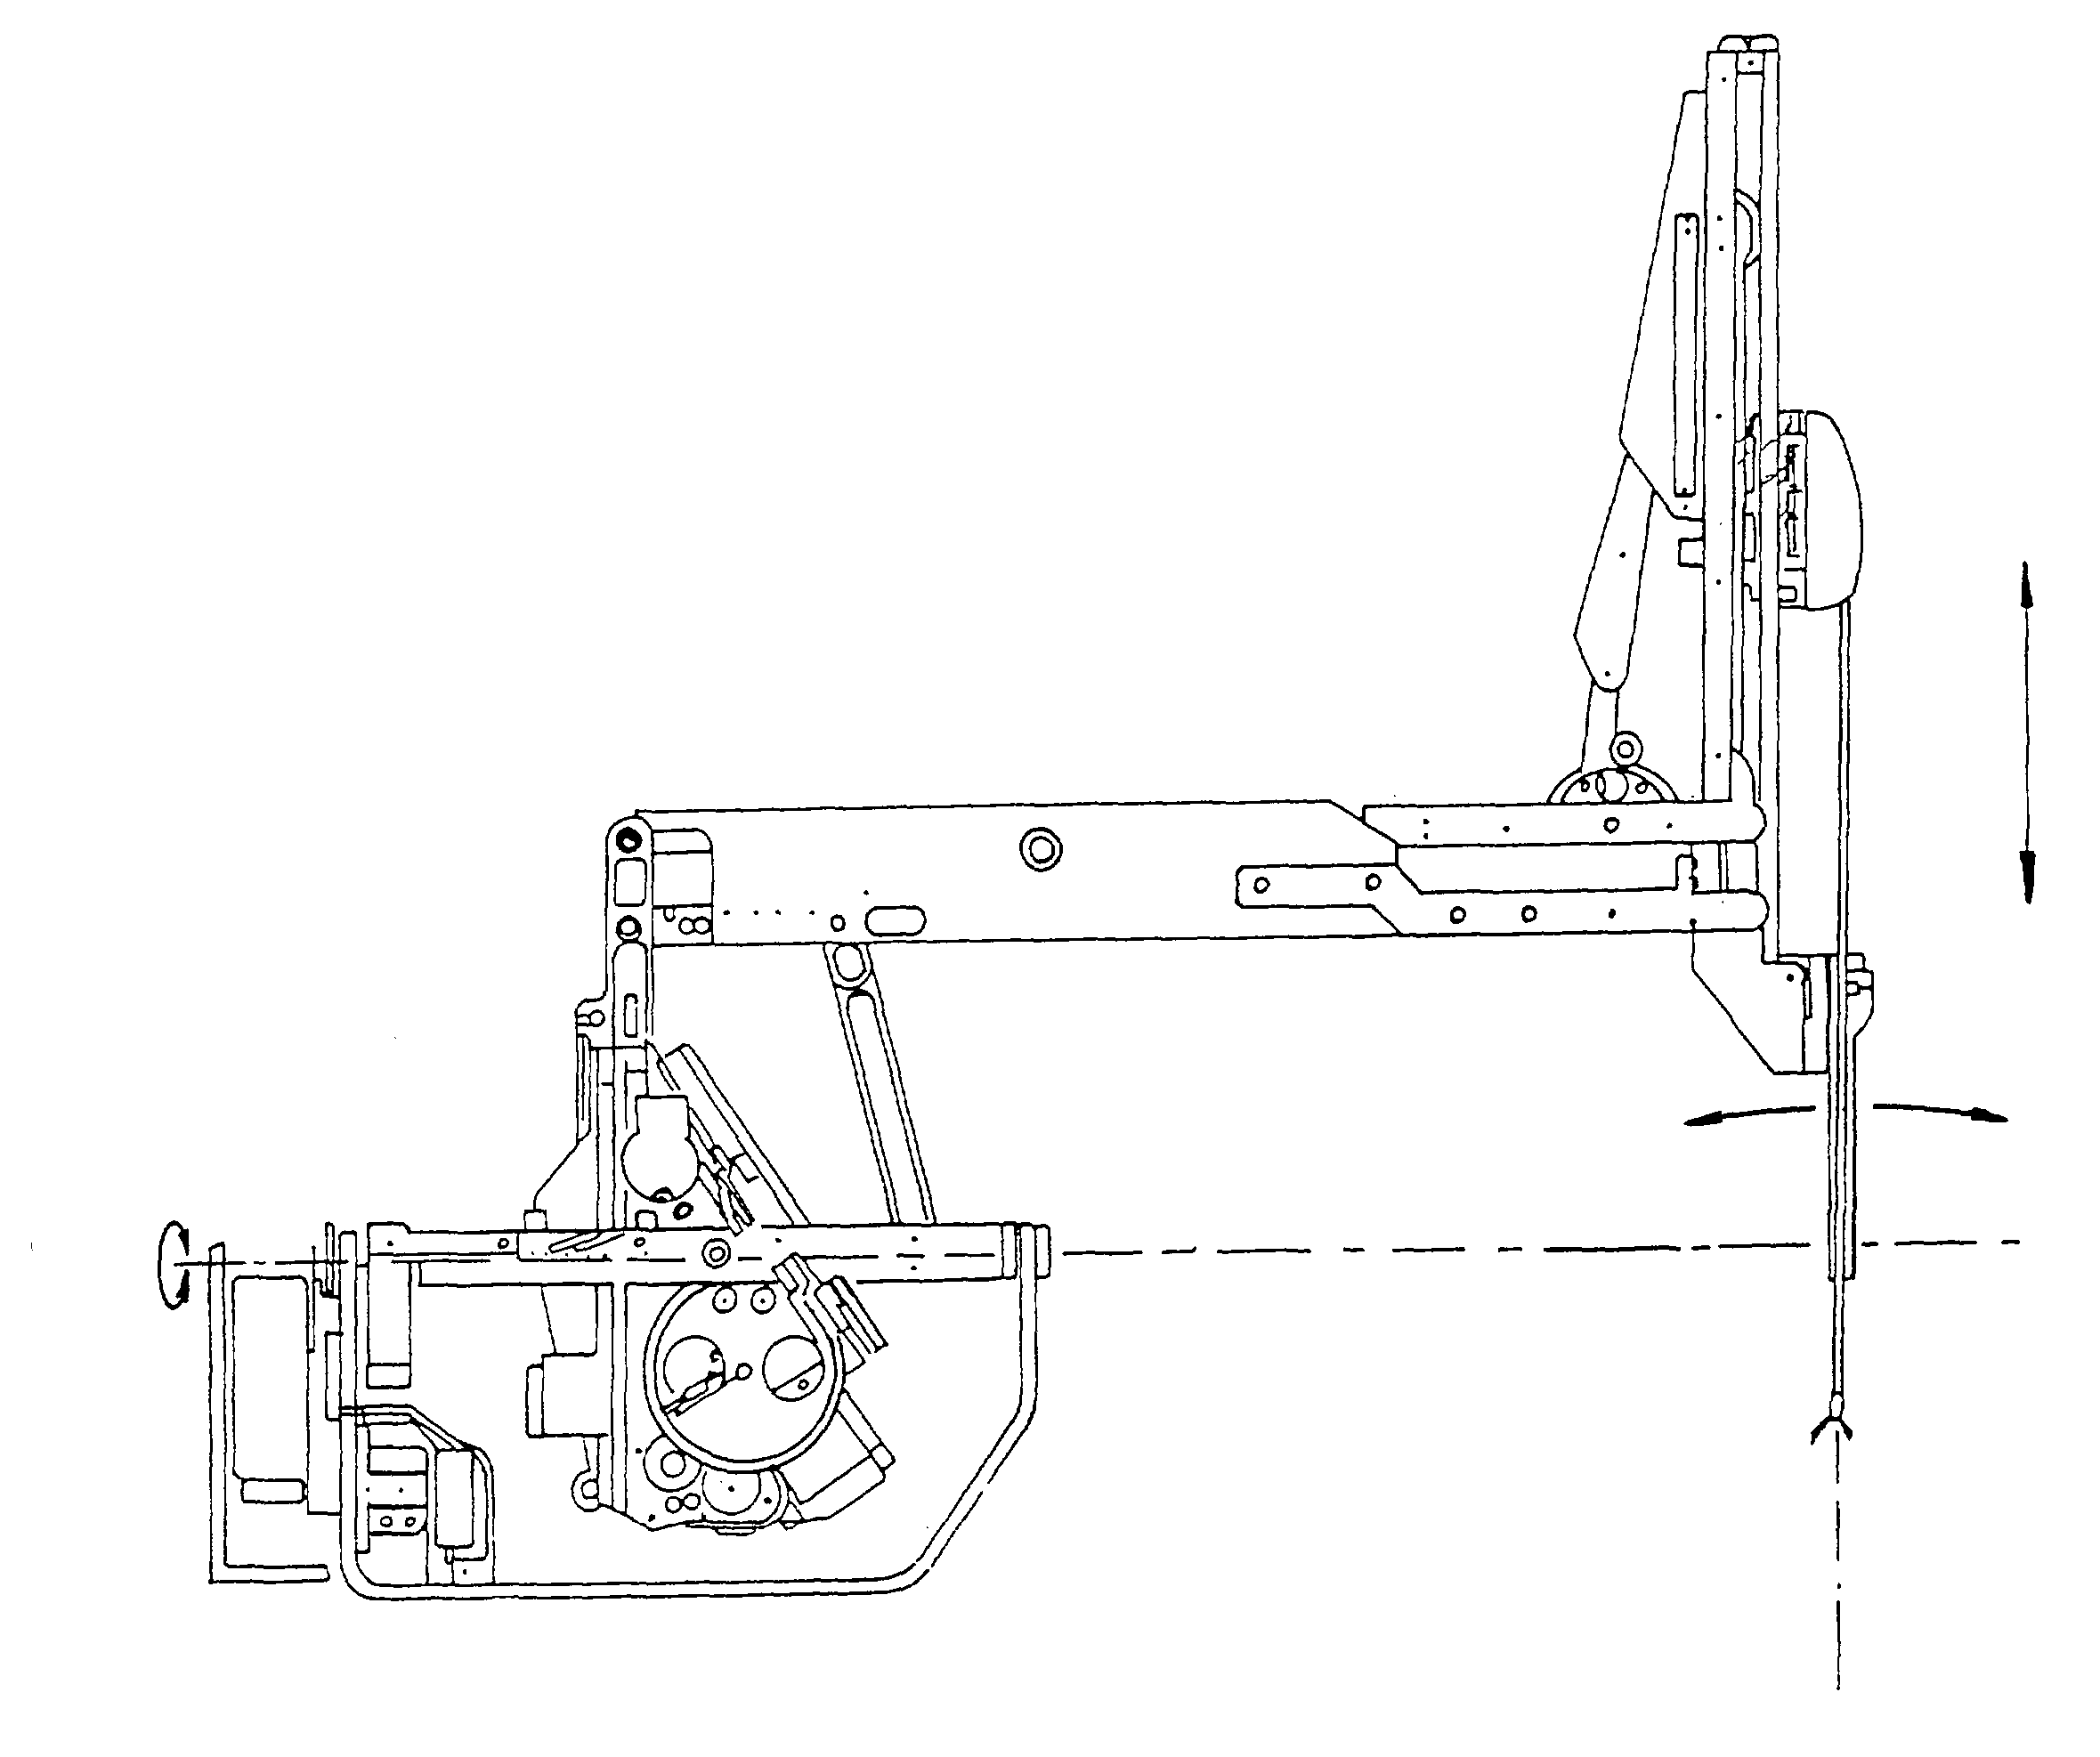
\includegraphics[width=0.7\unitlength]{graphics/US07865266-20110104-D00006-hand-cutout}}%
      \put(0.35,0.465){\scriptsize Parallel linkage}%
      \put(0.45,0.45){\vector(2,-3){0.07}}
      \put(0.55,0.065){\scriptsize Fulcrum point}%
      \put(0.65,0.09){\vector(4,3){0.08}}
    \end{picture}%
  \endgroup%
  \caption{Illustration of the da Vinci offset remote center manipulator~\cite{moll2011cooperative}. \label{fig:remote_center_manipulator}}
\end{figure}

\begin{figure}[t]
  \centering
  \begingroup%
    \setlength{\unitlength}{\linewidth}%
    \begin{picture}(1,0.6)%
      \put(0.25,0){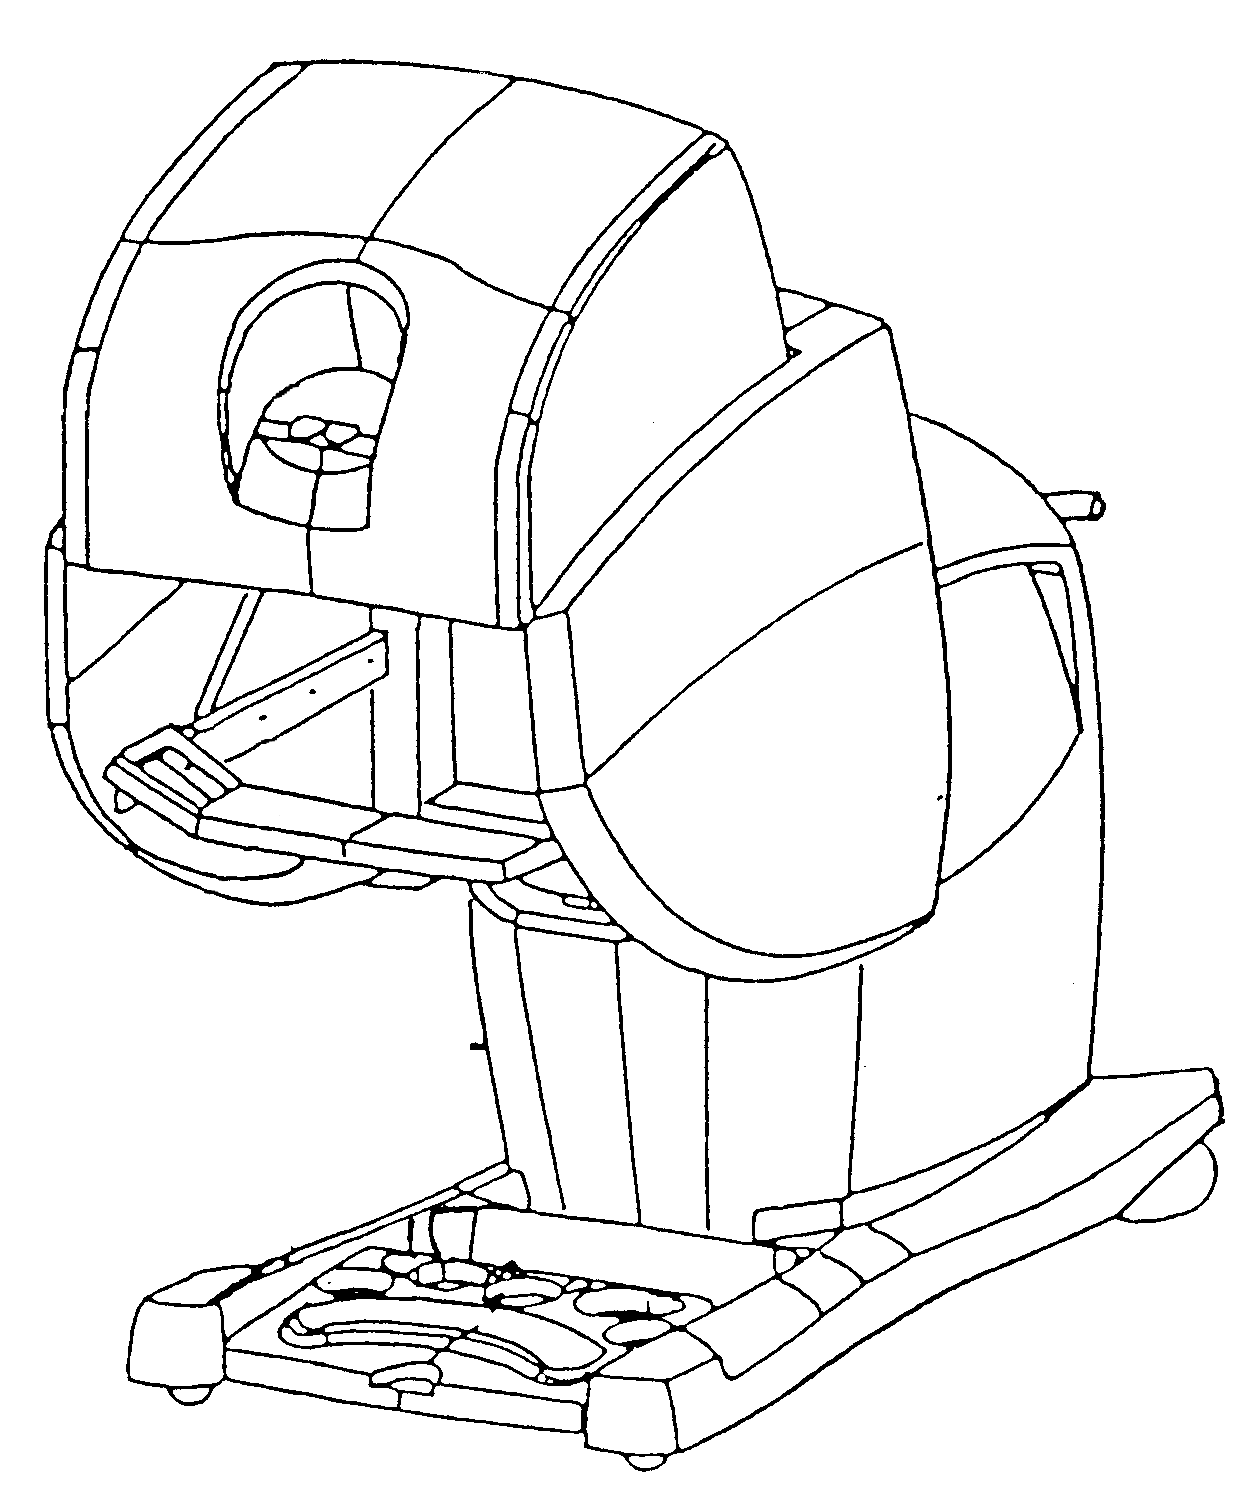
\includegraphics[width=0.5\unitlength]{graphics/US06714839-20040330-D00001-master-cutout}}%
      \put(0.095,0.495){\scriptsize Stereo display}%
      \put(0.2,0.48){\vector(3,-1){0.15}}
      \put(0.025,0.335){\scriptsize Auxiliary controls}%
      \put(0.13,0.32){\vector(4,-1){0.13}}
      \put(0.3,0.18){\scriptsize Joysticks}%
      \put(0.37,0.21){\vector(1,2){0.04}}
      \put(0.69,0.028){\scriptsize Pedals}%
      \put(0.68,0.035){\vector(-4,1){0.13}}
    \end{picture}%
  \endgroup%
  \caption{Illustration of the da Vinci master console~\cite{salisbury2004master}. \label{fig:console}}
\end{figure}

\subsection{Illustration of the surgery}
d
\subsection{Description of the robot}

\begin{figure}[t]
    \centering
       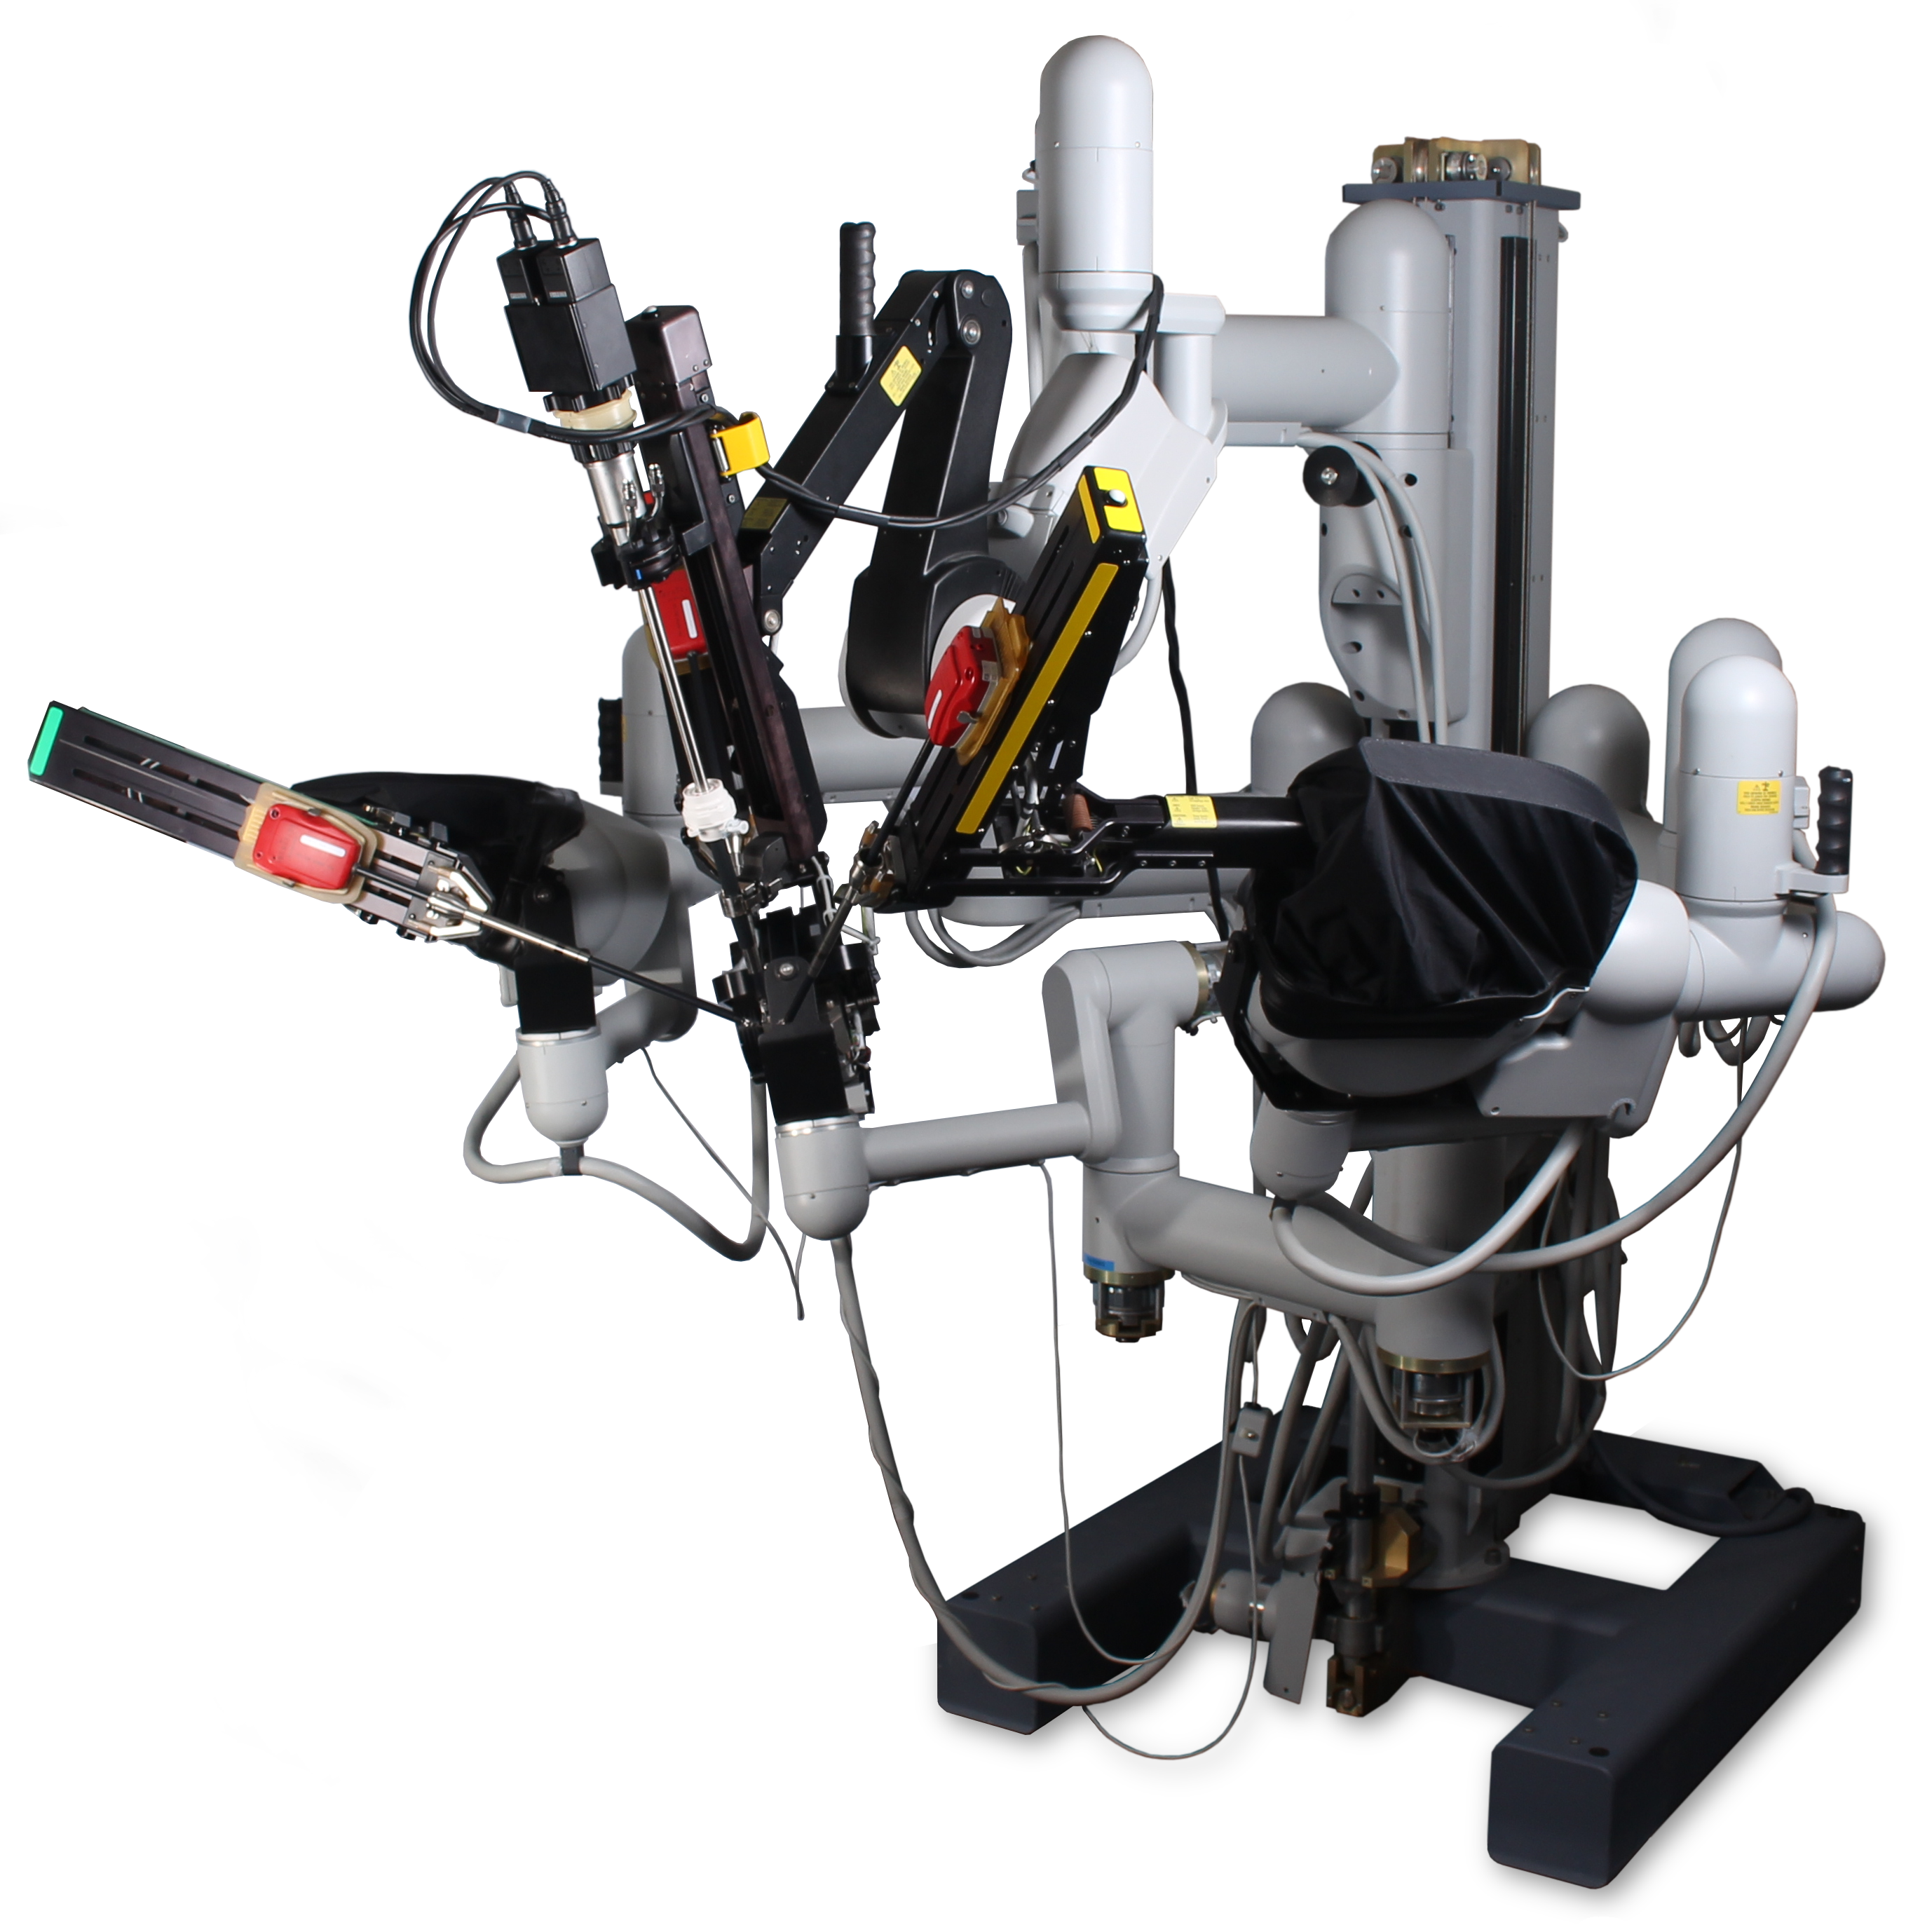
\includegraphics[width=0.7\linewidth]{graphics/patient_cart.png}
    \caption{The da Vinci surgery robot as it sits in the laboratory at Aalborg University. One arm is partially disassembled for easy access to the actuators and sensors. \label{fig:patient_cart}}
\end{figure}

% \begin{figure}
%     \centering
%        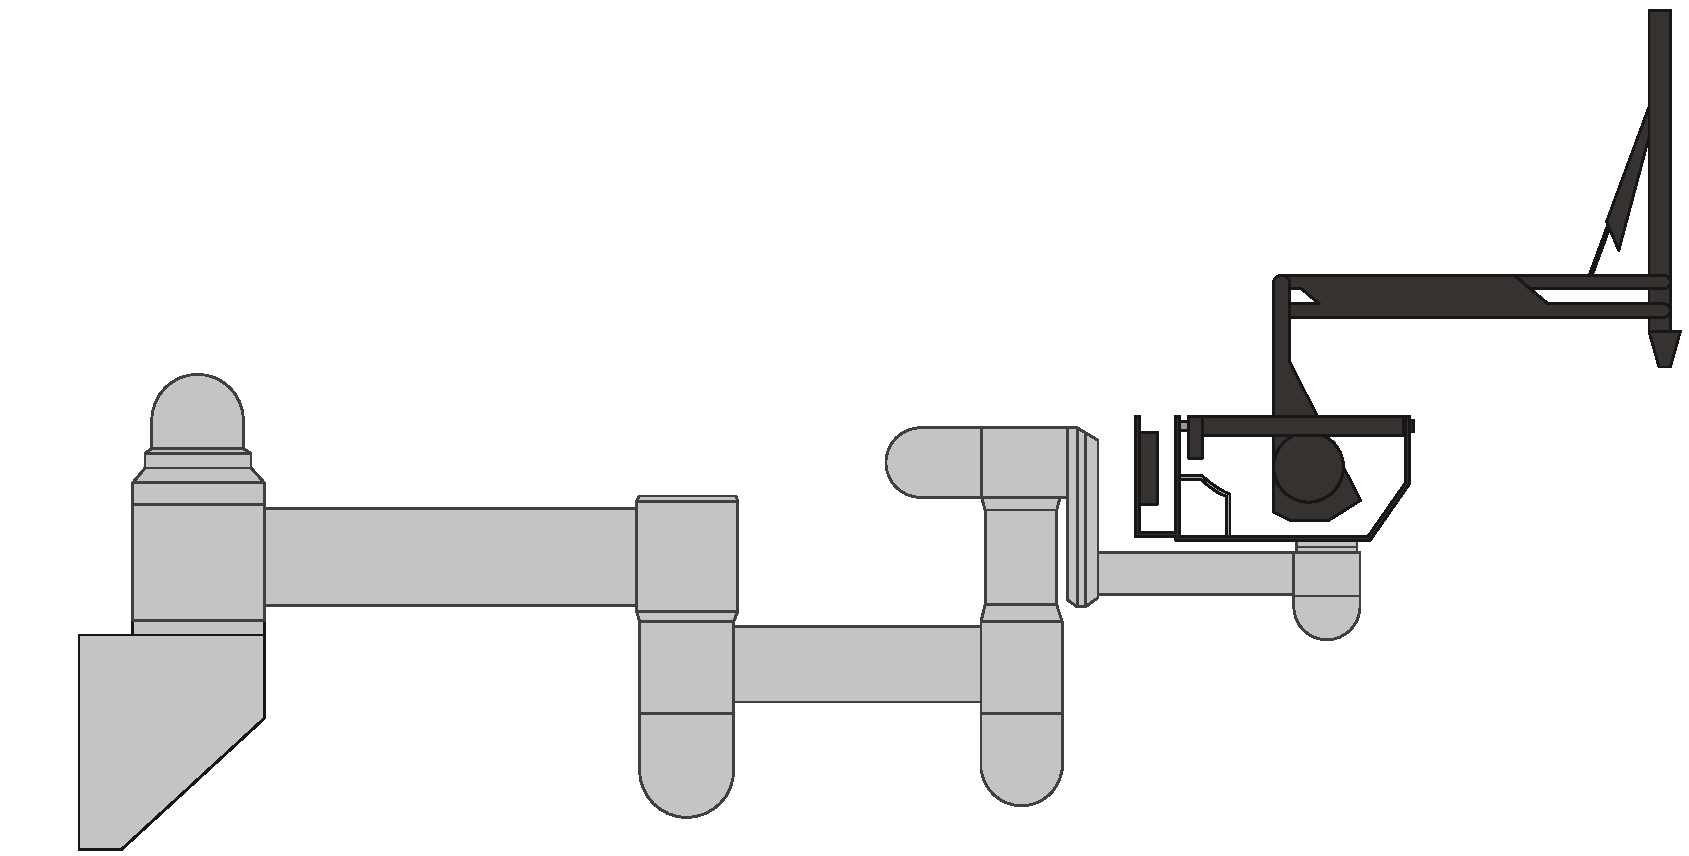
\includegraphics[width=0.8\linewidth]{graphics/p4-conceptual.pdf}
%     \caption{Sketch of one robot arm. The black manipulator part provides a remote fulcrum point via a parallel linkage.\label{fig:p4-conceptual}}
% \end{figure}

\begin{figure}[t]
    \centering
       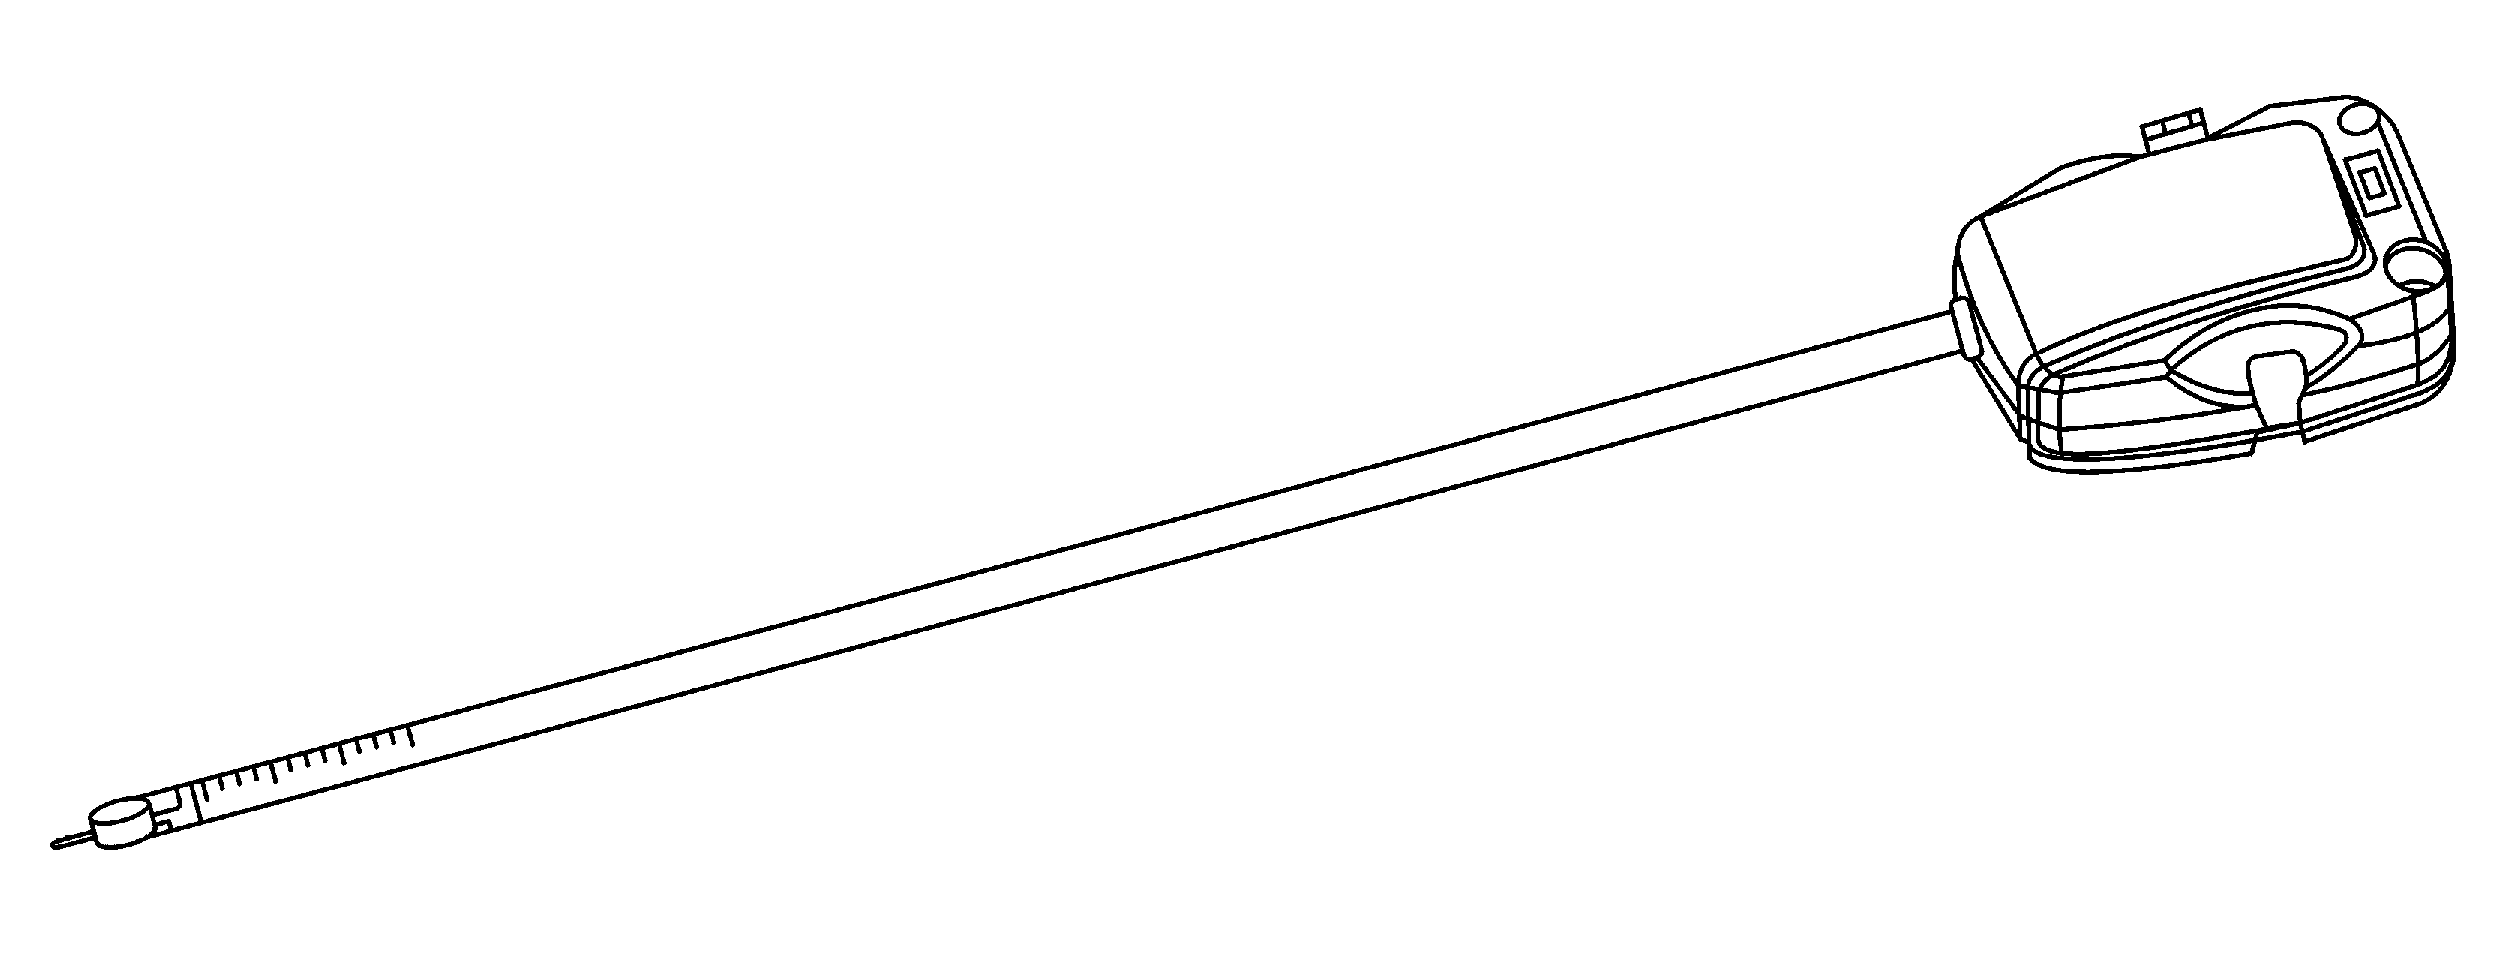
\includegraphics[width=0.8\linewidth]{graphics/US08834489-20140916-D00004-instrument-cutout}
    \caption{Drawing of an EndoWrist instrument. \label{fig:instrument}}
\end{figure}

\begin{figure}[t]
    \centering
       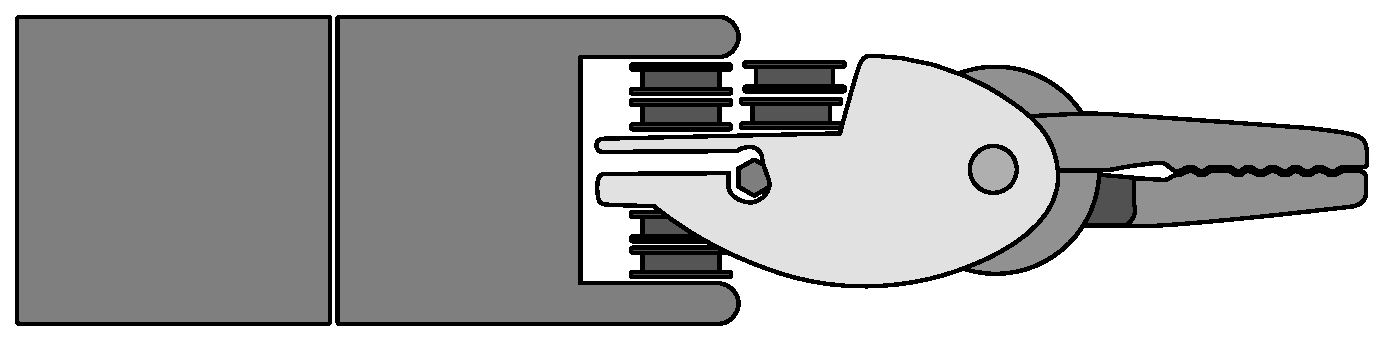
\includegraphics[width=0.8\linewidth]{graphics/Needle-driver_conceptual.pdf}
    \caption{Sketch of the tip of the needle-driver instrument. \label{fig:gripper_tip}}
\end{figure}

Type 118746 - http://www.maxonmotor.com/maxon/view/product/motor/dcmotor/re/re25/118746
\cleardoublepage
\subsection{Description of the system}
The AAU surgical robot is at present completely computer controlled; thus, the master console is not used. In stead of the console, a computer system has been build. 

%does not use the master console, however, uses only the patient cart by tapping into the connection to the console.
%A fair amount of reverse engineering has resulted in a system that is able to measure the state of the manipulator arms and control their servos.
%For modularity reasons, each arm has a dedicated control system.
%
%The systems consist of two embedded computers National Instruments single board RIO controllers, which has the two main tasks:
%\begin{itemize}
%\item Getting measurements (positions, velocities, motor currents) from the sensors on the arm and sending them to a client PC, and
%\item getting control reference signals from the PC to drive the motors that controls the motors.
%\end{itemize}
%A diagram of the system is shown in Figure~\ref{fig:hardwareRobot}. Beside these two tasks, the embedded computers enforce security constraints like limiting control values to protect the motors and stopping the motors when the joints reach their limits.




\subsubsection{Control system}
The control system is designed with a cascade structure consisting of three control loops, as shown in Fig.~\ref{fig:hardwareOverview}.
\begin{figure}[!ht]
\centering
  \def\svgwidth{\columnwidth}
\graphicspath{{graphics/}}
\begin{footnotesize}
\input{graphics/hardwareOverview.pdf_tex}
\end{footnotesize}
\caption{Association of control loops to physical hardware.}
\label{fig:hardwareOverview}
\end{figure}

The main idea of using a cascade control structure is to obtain disturbance attenuation and elimination of nonlinear effects. The dynamics of the end-effector joints are affected by a considerable friction; hence, cascade control of these joints is imperative to obtain a good performance. To obtain a large bandwidth, we implement the controls in hardware. In particular, the current and speed controllers are implemented in the ESCON motor driver, running at sampling frequencies of 54~kHz and 5.4~kHz, and the position controller is implemented in the FPGA with a sampling frequency of 2~kHz.

The current implementation of the control system allows a sampling frequency, which is comparable to the 1300~Hz of the da Vinci
surgeon console \cite{faust2007robotics}. This opens the possibility to do research on a surgical robot with performance comparable to a state-of-the-art commercial robot.

trajectory planning 100~Hz





%\input{graphics/hardwareOverview.pdf_tex}
%%\begin{figure}[t]
%%    \centering
%%       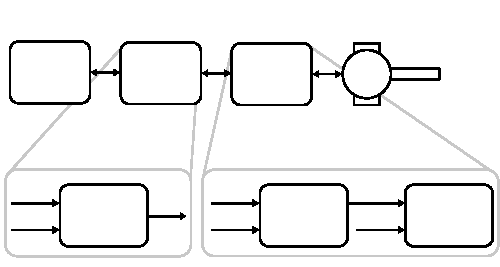
\includegraphics[scale=1]{graphics/hardwareOverview.pdf}
%%    \caption{TBD. \label{fig:hardwareOverview}}
%%\end{figure}
%\begin{center}
%\resizebox{\linewidth}{!}{\input{graphics/hardwareOverview.pdf_tex}}
%\end{center}

\subsection{Description of the ROS packages}

\subsection{Results on performance}

\subsection{Surgery open laboratory concept}
Robotic surgery requires real physical robots for experiments and to validate simulated models.
However, setting up a robotic surgery laboratory is expensive and space- and time-consuming.
Having set up the laboratory at Aalborg University, we will invite everybody interested to collaborate with us.
We are providing free access to our simulation model and control software to use in both education and research.
When the time comes to test the developed software, we will provide access to our lab, and are happy to cooperate all the way.

We believe that this open source philosophy is conducive to research, as has been shown by the success of ROS.

Furthermore, we would like to support any body who is interested in setting up similar laboratories.
As hospitals usually write of a da Vinci Surgical System in 5 years, several of these systems may be sitting in their dusty hallways and may be easily acquired by universities.
We will be happy to provide the axillary equipment to set up a system identical to ours in a non-profit fashion.

\section*{Acknowledgment}
This work was supported by Spar Nord Fonden.

\bibliographystyle{IEEEtran}
\bibliography{bibliography}

\end{document}
